%!TEX root = main.tex

\setbeamercolor{block alerted title}{fg=black,bg=norange} % Change the alert block title colors
\setbeamercolor{block alerted body}{fg=black,bg=black!4} % Change the alert block body colors


\begin{alertblock}{Results}
	
 \textbf{Theorem 1. (Inclusion)} It follows that $$\{\mathcal{N}\} \subset \{\mathcal{O}\} \subset \{\mathcal{G}\}.$$ \\
 \setlength\parindent{24pt}
 \indent Inclusion is the first and most important result to this generalization. For every $\mathcal{N}$ there exists an $\mathcal{O}$ such that $\mathcal{O} \simeq \mathcal{N}.$ \\[0.7cm]
  \setlength\parindent{0pt}


  \textbf{Theorem 2. (Universality) } Let $F: A \to B$ be a continuous operator between Banach spaces. For every $\epsilon > 0$, there exist a GANN
$$  \mathcal{G}_2: A 	 \xrightarrow{g \circ T_1} C \xrightarrow{g \circ T_2} B$$
such that for all $\xi$
$$ \| {C}(\xi) -  F(\xi) \| < \epsilon.$$ \\[0.7cm]


	\begin{figure}
		 	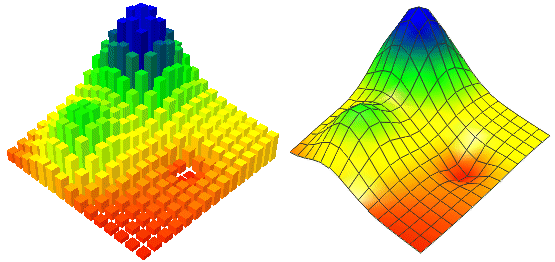
\includegraphics[width=0.6\onecolwid]{gc082_1.png}
		 	\caption{Parameter reduction using weight polynomials.}
	\end{figure}

\textbf{Theorem 3. (Parameter Reduction)} 
Let $\mathcal{C}$ be a continuous classifier
$$\mathcal{C}:  L^p(X) 	 \xrightarrow{g \circ \mathfrak{o}} L^q(Y) \xrightarrow{g \circ \mathfrak{n}_2}  \mathbb{R}^n.$$ with $O(1)$ weight polynomials.  If a continuous function, say $f(t)$ is sampled uniformly from $t = 0$, to $t = N$, such that $x_n = f(n)$,  then there exists a unique $\mathcal{N} \simeq \mathcal{C}$ with  $O(N^2)$ weights. \\[0.7cm]

\textbf{Generalized Backpropagation.} If $\mathcal{G}$ is parameterized by $W^{l} \in \mathbb{R}^{n\times m}$ then
\begin{equation*}
	B \otimes A \ni \frac{\partial \mathcal{G}}{\partial W^l} =
	   \underbrace{\left[\bigcomp_{k=L}^{l}  Dg \circ T_k\right]}_{\delta_{l+1}\text{ from BP}} \circ Dg \circ D\pi_l.
\end{equation*}

\end{alertblock}	


\begin{block}{References}
\footnotesize{
    \begin{thebibliography}{99} % Beamer does not support BibTeX so references must be inserted manually as below
        \bibitem[1]{p1} Burch, Carl (2012)
        \newblock A survey of machine learning
        \newblock \emph{International Conference on Artificial Intelligence and Statistics}
        \bibitem[2]{p1} Roux, Nicolas L and Bengio, Yoshua (2007)
        \newblock Continuous Neural Networks
        \newblock \emph{Journal of Machine Learning Research}
        
    \end{thebibliography}
}


 \end{block}
